\documentclass[11pt,a4paper,twocolumn]{article}

\usepackage[utf8]{inputenc} 
\usepackage{graphicx}
\usepackage{physics}
\usepackage{tikz}
\usepackage{listings}
\usepackage{xcolor}
\usepackage[toc, page]{appendix}
\usetikzlibrary{quantikz}     

\usepackage[
backend=biber,
style=alphabetic,
sorting=ynt
]{biblatex}
\addbibresource{sections/references.bib}

%%%%%%%% code color %%%%%%%%%%

\definecolor{codegreen}{rgb}{0,0.6,0}
\definecolor{codegray}{rgb}{0.5,0.5,0.5}
\definecolor{codepurple}{rgb}{0.58,0,0.82}
\definecolor{backcolour}{rgb}{0.95,0.95,0.92}

\lstdefinestyle{mystyle}{
    backgroundcolor=\color{backcolour},   
    commentstyle=\color{codegreen},
    keywordstyle=\color{magenta},
    numberstyle=\tiny\color{codegray},
    stringstyle=\color{codepurple},
    basicstyle=\ttfamily\footnotesize,
    breakatwhitespace=false,         
    breaklines=true,                 
    captionpos=b,                    
    keepspaces=true,                 
    numbers=left,                    
    numbersep=5pt,                  
    showspaces=false,                
    showstringspaces=false,
    showtabs=false,                  
    tabsize=2
}

\lstset{style=mystyle}

\title{\textbf{Quantum Research Project}}
\author{Pierriccardo Olivieri}
\date{March 2020}


\begin{document}
\pagenumbering{arabic}

\twocolumn[
  \begin{@twocolumnfalse}
    \maketitle
    \begin{abstract}
        
This project aims to analyze in a computer science perspective the quantum version of random walks: the quantum walks. This model of computation can be seen as a 
building block to construct new algorithms, here we are interested in a graph application in the domain of discrete time quantum walks. The question that this research 
want to answer is if a speedup w.r.t. classical is possible and discuss eventual limitations. 



    \end{abstract}
  \end{@twocolumnfalse}
  ]

\tableofcontents

\section{Introduction}

\subsection{Acronyms}

\begin{table}[h!]
\begin{tabular}{ll}
Acronym & Extended              \\
\hline
QW      & Quantum Walk          \\
DQWL    & Discrete QW on a Line \\
DTQW    & Discrete Time QW     
\end{tabular}
\end{table}

\subsection{Random Walks}

% random walk definition
A random walk, also known as a stochastic or random process, is a mathematical object which describe a path constituted by random step over a mathematical space. A common 
example is a random walk in a line. Consider the integer set Z, starting from a certain point, for instance x = 0, the path is defined by randomly choose to move left or 
right, the movement is achieved increasing or decreasing the value of x by 1. Tossing a coin will help in choosing randomly, with equal probability, the next step to take. 
This example could be generalized by increasing the dimension of the mathematical space considered, in a cartesian plane the starting point will have two  
coordinates and the possible moves becomes 4, and there are many other possible generalizations.

%random walk discrete and continuous
Random walks can be divided in two major classes, discrete-time and continuous-time random walk. Intuitively as the names suggest the difference between this two class 
is in the time function that could be integer or real, for a more formal definition consider the random walk as a system composed by a family of random variables ${X_{t}}$
the variables $X_{t}$ will measure the system at time t, now if we consider $t\in \mathbb{N}$  is a discrete-time stochastic process, otherwise if 
$t \in \mathbb{R}^{+} \bigcup \{0\}$ is a continuous-time stochastic process. 

% final
Here we focus on the discrete-time, in particular we bind this to graphs considering the random walk on a cyclic graph of order N.

\subsection{Quantum Walks}

The Quantum version of random walks is called Quantum Walks, also here there is a distinction between the two model of discrete quantum walks and 
continuous quantum walks, the focus of this research remain in the discrete-time domain also for the quantum side. 

Following the previous example of the random walk on a line here we discuss about a discrete quantum walk on a line called coined Discrete Quantum Walk on a Line (Coined DQWL), there are also versions without coin. It's worth introducing
the Coined DQWL in a formal and generic way, then apply to a more concrete example. A formal description starts considering the three main components of a Coined DQWL: 
A walker operator, a coin, an evolution operator usually called shift operator. 

% the walker
The Walker represents the position of our system and is defined in a Hilbert space infinite but countable $\mathcal{H}_{p}$, a vector in that space represents 
the position of the walker, $\ket{position} \in \mathcal{H}_{p}$ 

% the coin
The coin operator is defined in a two-dimension Hilbert space, if we consider as basis state $\ket{0}$ and $\ket{1}$ then the coin space becomes
$\mathcal{H}_{c} = { \ket{0}, \ket{1} }$ with $\ket{coin} \in \mathcal{H}_{c}$.

The complete system finally will be in a Hilbert space composed by the Kronecker product of the two spaces above defined 

\begin{equation}
    \mathcal{H}=\mathcal{H}_{p}\otimes\mathcal{H}_{c}
\end{equation}

A state of the coined DQWL can be defined by the vector:

\begin{equation}
    \ket{\phi_{initial}} = \ket{position}_{initial} \otimes \ket{coin}_{initial}
\end{equation}

% the evolution operator
The evolution operator, also called shift operator will actually perform a step starting from the initial position, apply this operator to the
system is equal to toss a coin and depending on the outcome move the walker to the left or to the right, we can do this by increment or decrement
the actual position by 1. A possible form of the shift operator could be described by this formula:

\begin{equation}
    \scriptstyle S = \ket{0}_{c} \bra{0} \otimes \sum{i} \ket{i + 1}_{p} \bra{i} + \ket{1}_{c} \bra{1} \otimes \sum{i} \ket{i - 1}_{p} \bra{i} 
\end{equation}

Finally we can see a walker as operator itself, called U and given by:

\begin{equation}
    U = S \times (C \otimes I_{p})
\end{equation}

Applying this operator to a given system is equal to perform a step of a random walk. This explanation derives from \cite{6812670} and \cite{Kempe_2003}.
The example on the following section apply this general concept to a cyclic graph.






\section{Coined Quantum Walk}

The following example shows how to implement a Coined discrete quantum walk on a cyclic graph with N = 8 nodes. This can be achieved using the coined DQW on a line
where the line is the cylic graph. First we need to encode the graph nodes in a binary notation to fit with qubits. In general a graph with $2^{n}$ nodes needs n encoding 
bit, in our case since we have $2^{3}$ nodes we can use 3 bit to encode. The Figure 1 below shows how we can bind the qubits to the nodes of the graph.

\begin{figure}[h!]
    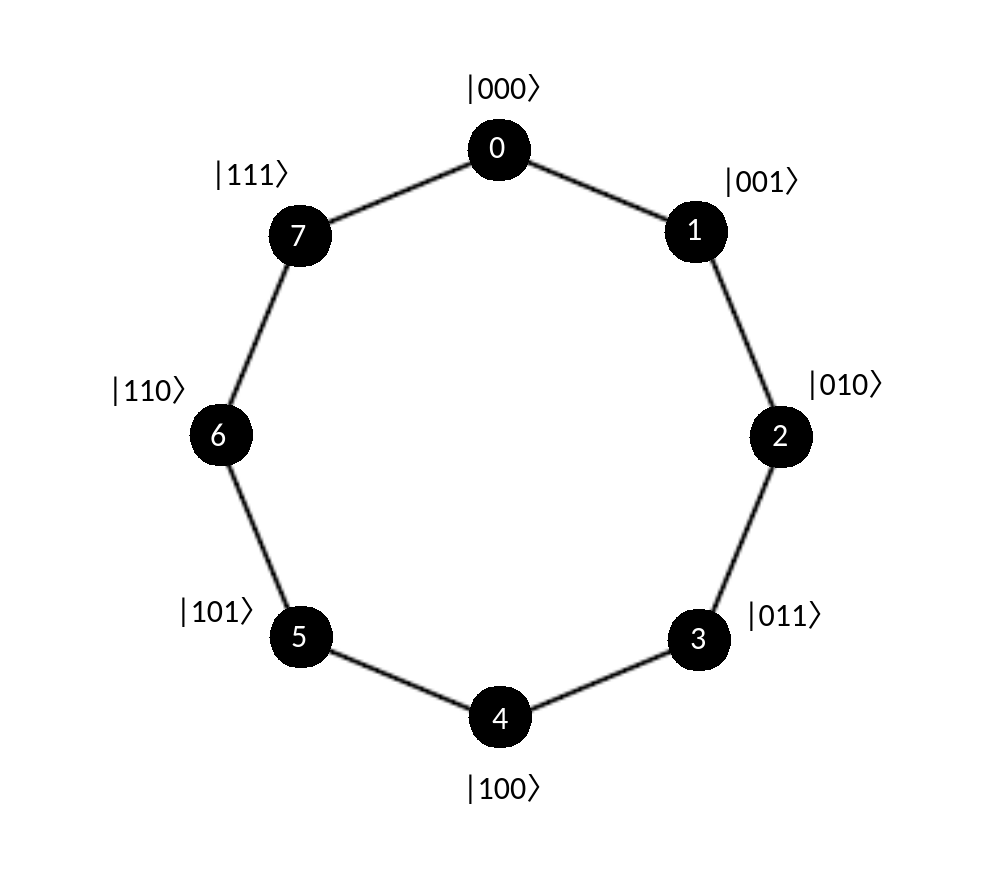
\includegraphics[scale=0.3]{img/cyclic_graph.png}
    \caption{Cyclic graph with 8 nodes, and the respective position state in qubits version}
    \centering
\end{figure}

\subsection{Components description}

We can fit now the 3 main components mentioned in the previous section for this specific example. 

% walker
Starting from the \textbf{walker operator}: for this version we need to encode the nodes of the graph in 3 qubits, usually we need log(N) qubits, in general this is not always true, 
we will see why in the next section. Using 3 qubits the postion of the walker is given by the binary encoding of the node, for instance the node 0 is represented as $\ket{000}$.

% coin operator
For the \textbf{coin operator} operator, we will use an Hadamard coin, that
consists in apply the Hadamard operator to the system. 

% hadamard coin description

% shift operator
The \textbf{shift operator} operator in this case will move the actual position that we call $\ket{i}$ to one of the adjiacent nodes, that corresponds to 
$\ket{i+1}$ or $\ket{i-1}$, which is decided by the outcome of the coin operator.

\subsection{Circuit for the CQW}

To implement the circuit in qiskit we need to translate the operator defined in quantum circuits, first we need 1 qubit for the coin and 3 for the position. 
The Hadamard can be easily implemented using an Hadamard gate on the first qubit. Then we need a circuit to perform an increment and a decrement on the initial state, 
this is less trivial and to achieve that we need two sub circuit that uses multi controlled toffoli gates. The circuit below represents an incrementer circuit 
for 3 qubits.

\begin{quantikz}
    & \ket{0} & \ctrl{2} & \ctrl{1} & \targ{}  & \qw \\
    & \ket{0} & \ctrl{1} & \targ{}  & \qw      & \qw \\
    & \ket{0} & \targ{}  & \qw      & \qw      & \qw \\
\end{quantikz}

The decrement circuit is similar but uses negative controlled not gates, the circuit below shows the decrement circuit for 3 qubits.

\begin{quantikz}
    & \ket{0} & \octrl{2} & \octrl{1} & \targ{}  & \qw \\
    & \ket{0} & \octrl{1} & \targ{}  & \qw      & \qw \\
    & \ket{0} & \targ{}  & \qw      & \qw      & \qw \\
\end{quantikz}

The negative controlled not can be represented by negate before and after the controlled not, the equivalence circuit below
clarify this explanation, for a detalied explanation look at \cite{nielsen_chuang_2010}.

$$
\begin{quantikz}[baseline={($(W.base)!.5!(W2.base) -height("$\vcenter{}$")*(0,1pt)$)}]
    & \octrl{1} & \alias{W}  \qw & \qw \\
    & \targ{}   & \alias{W2} \qw & \qw 
\end{quantikz}
=\begin{quantikz}[baseline={($(W.base)!.5!(W2.base) -height("$\vcenter{}$")*(0,1pt)$)}]
    & \gate{X}  & \ctrl{1} & \gate{X} & \qw \\
    & \qw       & \targ{}  & \qw      & \qw 
\end{quantikz}
$$

Finally the decrement circuit defined above, using this equivalence, is showed below.   

\begin{quantikz}
    & \ket{0} & \targ{} & \ctrl{2} & \ctrl{1} & \targ{} & \targ{} & \qw \\
    & \ket{0} & \targ{} & \ctrl{1} & \targ{}  & \qw     & \targ{} & \qw \\
    & \ket{0} & \targ{} & \targ{}  & \qw      & \qw     & \targ{} & \qw \\
\end{quantikz}

A similar implementation in detail is covered in \cite{douglas2007efficient}.
The final circuit by combining all the components defined is showed below.

\begin{quantikz}
    &\lstick{$\ket{0}$\\coin} & \ctrl{3} & \ctrl{2} & \ctrl{1}& \qw  & \targ{} & \ctrl{3} & \ctrl{2} & \ctrl{1} & \targ{} & \qw \\
    & \ket{0} & \ctrl{2} & \ctrl{1} & \targ{} & \qw  & \targ{} & \ctrl{2} & \ctrl{1} & \targ{}  & \targ{} & \qw \\
    & \ket{0} & \ctrl{1} & \targ{}  & \qw     & \qw  & \targ{} & \ctrl{1} & \targ{}  & \qw      & \targ{} & \qw \\
    & \ket{0} & \targ{}  & \qw      & \qw     & \qw  & \targ{} & \targ{}  & \qw      & \qw      & \targ{} & \qw \\
\end{quantikz}

It's worth to make some comments about it, this circuit represents the U operator, in fact the Hadamard coin will 
randomly choose the direction to take and activate the increment or decrement sub circuit. Therefore this corresponds
to a single iteration of the walk, by successively apply this circuit we can perform a random walk on the cyclic graph.
The code for this circuit can be found in the Appendix A at the end of this document.  


\section{Generalization and results}

The example shown above can be generalized in all aspects, let's start with the graph nodes.
We have considered for the eample a 8-node graph, but considering the generalized N-node version, are necessary
auxiliary qubits for creating multi controlled toffoli gates. Depending on the chosen mode
to implement the multi toffoli gate if the control bits are greater than 2 can be required 
a number of ancillary bits equal to the number of control quibits CQ - 1.

Another generalization concerns the type of graph, by modifying the circuit appropriately it is possible to
perform a random walk in different types of graphs including, glued trees, complete graphs etc. a 
detailed presentation of the various types of graphs with their circuit is present in \cite{douglas2007efficient}

Shift and Coin operators can also be generalized for various applications, for the Coin operator in
particular there are different forms with different properties, the Hadamard coin presented above shows a peculiarity
of the Quantum, one would also expect for the Quantum a Gaussian distribution of T-step node visits
as happens in the classic version, in reality the distribution obtained is asymmetrical. Figure 2 below shows that 
the results after T steps in the cyclic graph. More details about this behavior and alternatives 
symmetrical to the Hadamard coin can be found in \cite{Kempe_2003}

\section{Complexity and problem definition}

To talk about complexity in Quantum Walks we need to introduce the concept of Hitting Time. A definition can be found in \cite{6812670}
\\
\textbf{definition: Hitting Time}  



Now we can define the problem of searching for a marked vertex. Given the example proposed, using the Hadamard coin, of a 
cyclic graph with 8 nodes, to search for a marked vertex starting from given vertex we need to perform a walk in the graph 
and see if the current vertex is the one we are searching. The problem here is how often perform a measure, this choice
will impact also on the performances, indeed if we measure the circuit at each step we loose all the advantages of the quantum
coerenches and the performances will be equals to classical, we can gain some advantages by set the probability of measuring
very small \cite{Kempe_2003}.    
\printbibliography[title={References}]

\twocolumn[
  \begin{@twocolumnfalse}
    \appendix
    \section{Coined Quantum walk}
This code below is referred to coined quantum walk, using Hadamard coin for a
cycle graph with number of nodes N=3.
\enlargethispage{\baselineskip}

\begin{lstlisting}[breaklines,language=Python]
from qiskit import *

#increment operator for a 3-bit state register
def increment_op(circuit):
    qr = circuit.qubits
    circuit.mct([qr[0],qr[1],qr[2]],qr[3],None,mode='noancilla')
    circuit.ccx(qr[0],qr[1],qr[2])
    circuit.cx(qr[0],qr[1])
    circuit.barrier()
    return circuit

#decrement operator for a 3-bit state register
def decrement_op(circuit):
    qr = circuit.qubits
    circuit.x(qr)   
    circuit.barrier()
    circuit.mct([qr[0],qr[1],qr[2]],qr[3],None,mode='noancilla')
    circuit.ccx(qr[0],qr[1],qr[2])
    circuit.cx(qr[0],qr[1])
    circuit.barrier()
    circuit.x(qr)
    return circuit

#construct the circuit for one step of the random walk
def random_walk_step(circuit):
    #increment operator circuit
    qr_incr = QuantumRegister(4)
    increment_circ = QuantumCircuit(qr_incr, name='increment')
    increment_op(increment_circ)
    increment_inst = increment_circ.to_instruction()

    #decrement operator circuit
    qr_decr = QuantumRegister(4)
    decrement_circ = QuantumCircuit(qr_decr, name='decrement')
    decrement_op(decrement_circ)
    decrement_inst = decrement_circ.to_instruction()

    circuit.h(qr[0])
    circuit.append(increment_inst, qr[0:4])
    circuit.append(decrement_inst, qr[0:4])
    
    return circuit   

def random_walk(steps, circuit):
    for i in range(0, steps):
        random_walk_step(circuit)
    return circuit  

\end{lstlisting}
%\lstinputlisting[breaklines,breakatwhitespace,caption=inputenc,language=Python]{code/coined_quantum_walk.py}

  \end{@twocolumnfalse}
  ]
    
\end{document}